\chapter{Vector Fields and Integral Curves}
  \subsection*{A rough explanation of vector fields and integral curves}
    So far we have only dealt with $T_p(\mathcal{M})$, the vector space of
    all tangent vectors at a point $p \in \mathcal{M}$. In this section, we
    introduce another mathematical object known as a vector field $X$, which
    roughly speaking, assigns \textbf{one} tangent vector to each point $p$
    on a $C^\infty$ (i.e smooth) manifold $\mathcal{M}$ in a \textbf{smooth}
    manner\footnote{The meaning of smooth assignment will be explained more
    precisely later}. Different vector fields $X_1$, $X_2$ \dots etc are
    different assignments of tangent vectors to each point $p \in
    \mathcal{M}$.

    A familiar example would be the electric field in $\mathbb{R}^3$; to
    each point $p \in \mathbb{R}^3$, we have an electric field vector, which
    is an element of $T_p(\mathbb{R}^3)$ (which is a 3 dimensional real
    vector space). Different electric fields lead to different assignments of
    electric field vectors to all points in $\mathbb{R}^3$.

    Another way of thinking about vector fields would be to imagine a
    family of \textbf{non-intersecting} smooth curves that fill
    $\mathcal{M}$. Then, for each point on the manifold, we assign to it a
    vector that is tangent to the curve that is passing through that point.
    Such curves are known as integral curves.

    An example would be consider a magnetic field pointing straight up and
    changing with time. We know from undergraduate EM that the
    equipotential curves are just concentric circles, and the electric
    field at a point is tangent to the concentric circle passing through
    that point. The concentric circles are the integral curves, and the
    electric field is the vector field for those integral curves. 

    Now, let's see the precise meaning of all of the above.
  \subsection*{The precise definition of a vector field}
    \begin{definition}[Vector field]
      \label{defn: vector field}
      A vector field $X$ on a $C^\infty$ manifold is a smooth assignment of a
      tangent vector $X_p \in T_p(\mathcal{M})$ at each point
      $p\in\mathcal{M}$ where "smooth" is defined to mean that, for all $f\in
      C^\infty(\mathcal{M})$, the function \[Xf: \mathcal{M} \rightarrow \mathbb{R}\]
      defined by:
      \[p \rightarrow (Xf)(p) = X_p(f)\]
      is infinitely differentiable.
    \end{definition}
    \begin{remark}
      There is a lot to unpack in definition~\ref{defn: vector field}.
      Points~\ref{item: local chart vector field part 1}, \ref{item: local
      chart vector field part 2} are especially important, because
      definition~\ref{defn: vector field} will make a lot more sense once we
      go into a local chart.
      \begin{enumerate}
        \item{Notice how we wrote $X_p$ instead of $X^\sigma_p$. We don't
        write $\sigma$ here because in the past, $\sigma$ referenced an
        entire equivalence class of curves, where different $\sigma$ would
        give different tangent vectors at the point $p$, but now there is
        just \textbf{one} tangent vector at the point $p$, which is assigned
        by the vector field. If you really want to think about curves, then
        $X_p$ is the vector tangent to the integral curve at the point $p$.}
        \item{$X$ is a map from $C^\infty(\mathcal{M})$ to
          $C^\infty(\mathcal{M})$. Notice how $f \in C^\infty(\mathcal{M})$
          and $Xf \in C^\infty(\mathcal{M})$. To easily see why $Xf \in
          C^\infty(\mathcal{M})$,
          we can write $Xf = X_{(\,\,)}(f)$ such that:
          \begin{align*}
            Xf: \mathcal{M} \rightarrow& \mathbb{R}\\
            p \mapsto& X_{(p)}(f)
          \end{align*}}
        \item{\label{item: local chart vector field part 1}Consider a local chart
        $(U,\phi)$. Then, in this local chart, with $x = \phi(p) = (x^1,...,x^m)$, we have:
        \begin{equation}
          \label{eqn: local chart vector field}
          \begin{split}
          (Xf)(p) &= X_p(f) \\
          &= X^i(x) \frac{\partial}{\partial x^i}\Big(\bar{f}(x)\Big)\Bigr|_{x}
          \end{split}
        \end{equation}
        where $\bar{f} = f \circ \phi^{-1}$, and where we write $X^i(x)$ to
        remind ourselves that the components of $X_p$ in the local chart
        depend on $\phi(p) = x$, and we also write $\frac{\partial}{\partial
        x^i}\big(\bar{f}(x)\big)\Bigr|_{x}$ to show that this partial
        derivative is evaluated at the point $\phi(p) = x$.
        
        Thus, "smooth assignment of of a tangent vector $X_p \in
        T_p(\mathcal{M})$ at each point $p\in\mathcal{M}$" just means that
        the last line in equation~\ref{eqn: local chart vector field} is a
        smooth function of $x$ when we vary $x$. Varying $x$ simply means
        moving to another point $p$ on the manifold, because $x = \phi(p)$.
        In other words, we want \[X^i(x) \frac{\partial}{\partial
        x^i}\Big(\bar{f}(x)\Big)\Bigr|_{x}: \mathbb{R}^m \rightarrow
        \mathbb{R}\] to be an infinitely differentiable function of $x$.}
        \item{\label{item: local chart vector field part 2}Again, consider a
        local chart $(U, \phi)$, where $x = \phi(p)$. If we write
        \begin{equation*}
          (Xf)(p) = (Xf) \circ \phi^{-1} \circ \phi(p) \equiv \overline{Xf}(x)
        \end{equation*}
        we have, comparing with our work from point~\ref{item: local chart
        vector field part 1},
        \begin{equation*}
          \overline{Xf}(x) = X^i(x) \frac{\partial}{\partial
          x^i}\Big(\bar{f}(x)\Big)\Bigr|_{x}
        \end{equation*}
        Thus, we can write: 
        \begin{align*}
        \overline{X}: C^\infty(\mathbb{R}^m) &\rightarrow C^\infty(\mathbb{R}^m)\\
        \bar{f} &\mapsto \overline{Xf}  = X^i(\,\,) \frac{\partial}{\partial
        x^i}\Big(\bar{f}(\,\,)\Big)\Bigr|_{(\,\,)}
        \end{align*}
        where
        \begin{align*}
          \overline{Xf}:
          \mathbb{R}^m
          &\rightarrow \mathbb{R}\\
          x &\mapsto X^i(x) \frac{\partial}{\partial
          x^i}\Big(\bar{f}(x)\Big)\bigr|_{x}
        \end{align*}
        Thus, we see that the local representation of $X$ in a coordinate
        chart is \[\overline{X} = X^i(\,\,) \frac{\partial}{\partial x^i}\]
        I.e, just like how $X$ takes in a point $p \in \mathcal{M}$ and returns a tangent vector $X_p$ at the point $p \in \mathcal{M}$, 
        $\overline{X}$ takes in $x =\phi(p) \in \mathbb{R}^m$ and returns a
        tangent vector $X^i(x) \frac{\partial}{\partial x^i}$ at the point $x
        \in \mathbb{R}^m$, where $X^i(x) \frac{\partial}{\partial x^i}$ is a smooth function of $x$.}
      \end{enumerate}
    \end{remark}
  \subsection*{The vector space of all vector fields
    $\mathcal{X}(\mathcal{M})$}
    Let $\mathcal{X}(\mathcal{M})$ be the set of all vector fields on the
    manifold $\mathcal{M}$. For $X,Y \in \mathcal{X}(\mathcal{M})$ and
    $\alpha \in \mathbb{R}$, we define the addition operator between two vector fields and the scalar multiplication operation as:
    \begin{subequations}
      \label{eqn: vector space of all vector fields operations}
      \begin{gather}
        (X + Y)f = X(f) + Y(f) \\
        (\alpha X)(f) = \alpha (X(f))
      \end{gather}
    \end{subequations}
    $\forall f\in C^\infty(\mathcal{M})$. From definition~\ref{defn:
    vector field}, since the addition of two tangent vectors at a point
    give a third tangent vector at a point, it is clear that
    $\mathcal{X}(\mathcal{M})$ together with the operations defined in
    equations~\ref{eqn: vector space of all vector fields operations} has a
    vector space structure.

    Thus, we shall denote $\mathcal{X}(\mathcal{M})$ as the vector space of all vector fields on the manifold $\mathcal{M}$.

    It is also meaningful to define the multiplication of a function $f \in
    C^\infty(\mathcal{M})$ with a vector field $X \in
    \mathcal{X}(\mathcal{M})$. I.e:
    \begin{align*}
    f\cdot X: C^\infty(\mathcal{M}) \rightarrow& C^\infty(\mathcal{M}) \\
    g\mapsto&
    (f\cdot X)(g)\\
    &\equiv f\cdot X(g)
    \end{align*}
    where $f\cdot X(g) \in C^\infty(\mathcal{M})$ is a map from
    $\mathcal{M}$ to $\mathbb{R}$, i.e \[ \left(f\cdot X(g)\right)(p) =
    f(p)\cdot(Xg)(p)\]
  \subsection*{Vector fields as derivations}
    From definition~\ref{defn: vector field}, we see that the map $X: C^\infty(\mathcal{M}) \rightarrow C^\infty(\mathcal{M})$ has all the properties of a derivation, since each $X_p$ is a derivation. These properties are:
    \begin{subequations}
      \begin{gather}
      X(f+g) = X(f) + X(g) \\
      X(rf) = r X(f) \\
      X(f\cdot g) = f\cdot X(g) + g\cdot X(f) \label{eqn:vector field leibniz rule}
      \end{gather}
    \end{subequations}
    where $f,g \in C^\infty(\mathcal{M})$, $r \in \mathbb{R}$.
  \section{Lie algebra structure}
    Now, we ask ourselves: can two vector fields be multiplied together to
    give a third field? Since each $X \in \mathcal{X}(M)$ is a map from
    $C^\infty(\mathcal{M})$ to $C^\infty(\mathcal{M})$, it seems reasonable
    to define the multiplication of two fields $X,Y$ as $X \cdot Y \equiv X \circ Y$, where $\forall f \in C^\infty(\mathcal{M})$, we have:
    \begin{equation}
      \label{eqn: bad vector field multiplication part 1}
      X \circ Y(f) = X(Y(f))
    \end{equation}
    However, equation~\ref{eqn: bad vector field multiplication part 1} is
    a bad definition, because $X\circ Y$ is not a vector field; $X\circ Y$
    fails to satisfy one of the properties of derivations, namely
    equation~\ref{eqn:vector field leibniz rule}.
    I.e, if $X\circ Y$ were a vector field, we should expect:
    \begin{equation*}
      [X\circ Y] (f\cdot g) = f\cdot [X\circ Y](g) + g \cdot [X\circ Y](f)
    \end{equation*}
    But instead, we have:
    \begin{align}
      [X\circ Y] (f\cdot g) &= X(Y(f\cdot g)) \nonumber \\
      &= X(f\cdot Y(g) + g\cdot Y(f)) \nonumber \\
      &= X(f\cdot Y(g)) + X(g\cdot Y(f)) \nonumber \\
      &= f\cdot X(Y(g)) + Y(g)\cdot X(f) + g\cdot X(Y(f)) + X(g) \cdot Y(f)\nonumber  \\
      &= f\cdot [X\circ Y](g) + g \cdot [X\circ Y](f) + \Big\{Y(g)\cdot X(f) +
      X(g) \cdot Y(f) \Big\} \label{eqn: bad vector field multiplication part 2}
    \end{align}
    We see the two extra terms at the end $Y(g)\cdot X(f)$ and
    $X(g) \cdot Y(f)$ prevent $[X\circ Y]$ from being a vector field.

    However, we can easily get rid of the last two terms; if we repeat the
    same calculations we did to arrive at equation~\ref{eqn: bad vector
    field multiplication part 2}, but for $[Y\circ X]$, we would arrive at:
    \begin{equation}
      \label{eqn: bad vector field multiplication part 3}
      [Y\circ X] (f\cdot g) = f\cdot [Y\circ X](g) + g \cdot [Y\circ X](f) + \Big\{Y(g)\cdot X(f) +
      X(g) \cdot Y(f) \Big\}
    \end{equation}
    Then, subtracting equation~\ref{eqn: bad vector field multiplication
    part 3} from equation~\ref{eqn: bad vector field multiplication part
    2}, we obtain:
    \begin{equation}
      \label{eqn: good vector field multiplication}
      [X,Y](f.g) = f[X,Y](g) + g[X,Y](f)
    \end{equation}
    where we have defined 
    \begin{equation}
      \label{eqn: commutator defn}
      [X,Y] \equiv X\circ Y - Y \circ X
    \end{equation}
    $[X,Y]$ is known as the commutator of the two vector fields $X,Y$. It
    is also called the Lie Bracket, for reasons that will become more clear
    when we talk about the Lie Derivative.

    Thus, we see from equation~\ref{eqn: good vector field multiplication}
    that while $X \circ Y$ and $Y \circ X$ aren't vector fields because
    they don't satisfy equation~\ref{eqn:vector field leibniz rule}, the
    commutator $[X,Y]$ is a vector field because it does (we can also
    easily show that the commutator satisfies all the other properties of a
    derivation). Now, let's see what the commutator looks like in a local chart $(U,\phi)$.
    \subsection{The commutator $[X,Y]$ in a local chart $(U, \phi)$}
      Consider a local chart $(U, \phi)$. Then, $\forall f \in
      C^\infty(\mathcal{M})$, $\forall p \in M$, we can write
      \begin{align*}
        \Big([X,Y](f)\Big)(p) &= \Big([X,Y](f)\Big) \circ \phi^{-1} \circ
        \phi(p) \\
        &= \overline{[X,Y](f)}(x)
      \end{align*}
      where $x = \phi(p)$ and $\overline{[X,Y](f)} = \big([X,Y](f)\big)
      \circ \phi^{-1}$ Now, we have:
      \begin{align*}
        \overline{[X,Y](f)}(x) =& \overline{[X(Y(f)) - Y(X(f)]}(x) \\
        =& \overline{X(\mspace{-10mu}\underbrace{Y(f)}_{\bar{k}\in
          C^\infty(\mathbb{R}^m)}\mspace{-10mu})}(x) -
          \overline{Y(\mspace{-10mu}\underbrace{X(f)}_{\bar{h}\in
          C^\infty(\mathbb{R}^m)}\mspace{-10mu})}(x) \\
        =& \overline{X(k)}(x) - \overline{Y(h)}(x) \\
        =& X^i(x)\frac{\partial}{\partial x^i}(\bar{k}) -
        Y^i(x)\frac{\partial}{\partial x^i}(\bar{h}) \\
        =& X^i(x)\frac{\partial}{\partial x^i}\left( Y^j(x)
        \frac{\partial\bar{f}(x)}{\partial x^j}\right) -
        Y^i(x)\frac{\partial}{\partial x^i}\left( X^j(x)
        \frac{\partial\bar{f}(x)}{\partial x^j}\right) \\
        =& X^i(x)\left(\frac{\partial \bar{f}(x)}{\partial x^j}\frac{\partial
        Y^j(x)}{\partial x^i} + Y^j(x)\frac{\partial^2 \bar{f}(x)}{\partial x^i \partial
        x^j}\right) - \\
        &Y^i(x)\left(\frac{\partial \bar{f}(x)}{\partial
        x^j}\frac{\partial X^j(x)}{\partial x^i} + X^j(x)\frac{\partial^2
        \bar{f}(x)}{\partial x^i \partial x^j}\right) \\
        =& \left(X^i(x) \frac{\partial Y^j(x)}{\partial x^i}
        \frac{\partial}{\partial x^j} - Y^i(x) \frac{\partial
        X^j(x)}{\partial x^i} \frac{\partial}{\partial x^j}\right)\bar{f}(x)
      \end{align*}
      Thus, we see that $\overline{[X,Y]}$ can be written as:
      \begin{equation}
        \label{eqn: commutator in local chart}
        \left(X^i \frac{\partial}{\partial x^i}Y^j - Y^i
        \frac{\partial}{\partial x^i}X^j\right) \frac{\partial}{\partial x^j}
      \end{equation}
    \subsection{Properties of the commutator $[X,Y]$}
      Clearly, from the definiton of the commutator in equation~\ref{eqn:
      commutator defn}, we have:
      \begin{subequations}
        \begin{gather}
          [X,Y] = -[Y,X] \\
          [X,[Y,Z]] + [Z,[X,Y]] + [Y,[Z,X]] = 0 \label{eqn: Jacobi identity}
        \end{gather}
      \end{subequations}
      where $X,Y,Z \in \mathcal{X}(\mathcal{M})$. By the way,
      equation~\ref{eqn: Jacobi identity} is known as the Jacobi
      identity.\footnote{Equation~\ref{eqn: Jacobi identity} is proved in
      the tutorials.}

      Now, the above two properties are essential elements in the structure
      of a Lie algebra. Formally, a Lie algebra is defined to be a real
      vector space $\mathcal{L}$ with a bilinear map $\mathcal{L} \times
      \mathcal{L} \rightarrow \mathcal{L}$ denoted by $(A,B) \mapsto [A,B]$
      which satisfies the following conditions:
      \begin{enumerate}
        \item{$\forall A,B \in \mathcal{L}$, \[[A,B] = - [B,A]\]}
        \item{$\forall A,B,C \in \mathcal{L}$, \[[A,[B,C]] +[C,[A,B]] +
        [B,[C,A]] = 0\]}
      \end{enumerate}
      We will come back to this when we discuss Lie groups and their associated tangent spaces.
  \section{Mapping of Vector Fields}
    \label{sec: mapping of vector fields}
    In section~\ref{sec: push forward between tangent spaces}, we
    saw how a differentiable map $\mathcal{F}: \mathcal{M} \rightarrow
    \mathcal{N}$ induces a map $\mathcal{F}_{*}:T_p(\mathcal{M})
    \rightarrow T_p(\mathcal{N})$ known as the push-forward map.
    \subsection*{Question: does $\mathcal{F}$ also induce a map from
    $\mathcal{X}(\mathcal{M})$ to $\mathcal{X}(\mathcal{N})$?}
      A natural way to define this induced map would be:
      \begin{equation}
        \label{eqn: attempt at defining induced map}
        \left(\mathcal{F}_{*}X\right)_{\mathcal{F}(p)} =
        \mathcal{F}_{*}(X_p)
      \end{equation}
      I.e, we define a vector field $Y = \mathcal{F}_{*}X$ in $\mathcal{N}$
      such that at the point $\mathcal{F}(p) \in \mathcal{N}$, there is a
      vector $\mathcal{F}_{*}(X_p) \in T_{\mathcal{F}(p)}(\mathcal{N})$.
      Now, equation~\ref{eqn: attempt at defining induced map} if a good attempt at defining this induced map, but it fails for two reasons:
      \begin{enumerate}
        \item{If $\mathcal{F}$ is not injective, then there might be two
        different points, $p_1,p_2 \in \mathcal{M}$ that map to the same
        point in $\mathcal{N}$, i.e $\mathcal{F}(p_1) = \mathcal{F}(p_2)$.
        In this case, should the induced vector at $\mathcal{F}(p_1) =
        \mathcal{F}(p_2)$ be $\mathcal{F}_{*}(X_{p_1})$, or
        $\mathcal{F}_{*}(X_{p_2})$?}
        \item{If $\mathcal{F}$ is not surjective, then $\exists p \in
        \mathcal{N}$ that don't have a pre-image in $\mathcal{M}$. How then
        should we assign a vector to $p\in \mathcal{N}$?}
      \end{enumerate}
      \begin{figure}
        \centering
        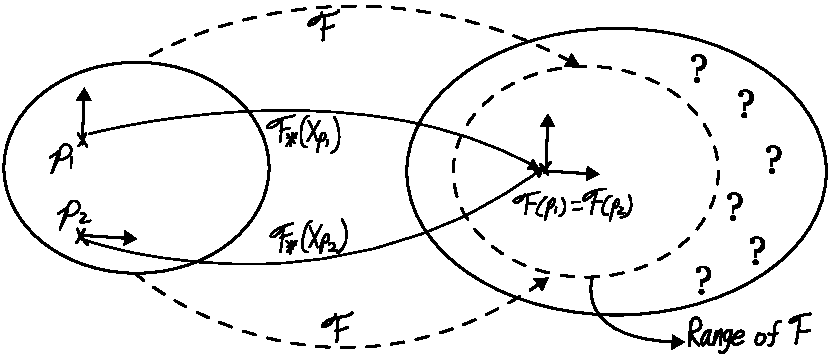
\includegraphics[width=0.7\textwidth, trim={0cm 0cm 0cm 0cm},clip]{push forward fail}
        \caption[]{}
        \label{fig: push forward fail}
      \end{figure}
      These two reasons are summarised in Figure~\ref{fig: push forward
      fail}. In summary, if $\mathcal{F}$ is not bijective (i.e if
      $\mathcal{F}$ is not a diffeomorphism), then $\mathcal{F}$ does not
      induce a map between $\mathcal{X}(\mathcal{M})$ and
      $\mathcal{X}(\mathcal{N})$.

      However, if $\mathcal{F}$ is a diffeomorphism, then the definition in
      equation~\ref{eqn: attempt at defining induced map} would be good,
      and $\mathcal{F}$ does indeed induce a map between
      $\mathcal{X}(\mathcal{M})$ and $\mathcal{X}(\mathcal{N})$. Let's put this in precise terms.
      
    \subsection{$\mathcal{F}$ related fields}
      \begin{definition}[$\mathcal{F}$ related fields\footnote{This
      definition is different from Kuldip's and is orignal...there might
      be some bugs.}]
        Let $\mathcal{F}: \mathcal{M} \rightarrow \mathcal{N}$ be a
        diffeomorphism, and let $X \in \mathcal{X}(\mathcal{M})$. Then,
        the diffeomorphism $\mathcal{F}$ induces a $\mathcal{F}$- related
        field $Y \in \mathcal{X}(\mathcal{N})$ by the following
        prescription:
        \[Y_{\mathcal{F}(p)} = \mathcal{F}_{*}(X_p)\]
        $\forall p \in \mathcal{M}$.

        We can write, $Y = \mathcal{F}_{*}\left(X\right)$ for the two
        $\mathcal{F}$-related vector fields $X,Y$.
      \end{definition}
      \remark{Informally, we shall say that the vector field $Y$ is the
      push-forward of the vector field $X$.}
      % , though strictly speaking this
      % is loose language (the push forward map is defined between tangent
      % spaces, but here we are only pushing forward one vector in the
      % tangent space of $p$ to give us another vector in the tangent space
      % of $\mathcal{F}(p)$).}
    \subsection{Some properties of $\mathcal{F}$ related fields}
      \begin{theorem}
        \label{theorem: f-related field calculation}
        Let $\mathcal{F}: \mathcal{M} \rightarrow \mathcal{N}$ be a
        diffeomorphism. If $X\in \mathcal{X}(\mathcal{M})$ and $Y\in
        \mathcal{X}(\mathcal{N})$ are $\mathcal{F}$-related, then
        $\forall f\in C^\infty(\mathcal{N})$, \[X\left(f \circ
        \mathcal{F}\right) = Y(f) \circ \mathcal{F}\]
      \end{theorem}
      \begin{remark}
        Given $p \in \mathcal{M}$, we can write theorem~\ref{theorem: f-related field calculation} in the following form:
        \[[X\left( f\circ \mathcal{F} \right)](p)= [Y(f)]\left(\mathcal{F}(p)\right)\]
        Remember that $f\circ \mathcal{F} \in C^\infty(\mathcal{M})$,
        and thus $X$ maps $f\circ \mathcal{F}$ to another function in $C^\infty(\mathcal{M})$.
      \end{remark}
      \begin{remark}
        Theorem~\ref{theorem: f-related field calculation} is very
        important. Given $X \in \mathcal{M}$, we can use
        theorem~\ref{theorem: f-related field calculation} to actually
        calculate $Y$. I.e, we can express the components of $Y$ in
        some local chart $(V,\psi)$ of $\mathcal{N}$ in terms of the
        components of $X$ in some local chart $(U,\phi)$ of
        $\mathcal{M}$. We will see how this works in
        corollary~\ref{corollary: f-related field calculation}.
      \end{remark}
      \begin{remark}
        Theorem~\ref{theorem: f-related field calculation} is the most important and the most powerful result of this section. All the other theorems in this section can be very easily proved by using this theorem.
      \end{remark}
      \begin{proof}[Proof of Theorem~\ref{theorem: f-related field
      calculation}]
        We begin by restating equation~\ref{eqn: important push forward
        result} which was derived in subsection~\ref{subsec:
        calculating a push-forward of a tangent vector}. For a
        diffeomorphism $\mathcal{F}:\mathcal{M} \rightarrow
        \mathcal{N}$, we have, $\forall f \in C^\infty(\mathcal{N})$,
        \begin{align*}
          W^{\sigma^\prime}_{\mathcal{F}(p)}(f) &\equiv
          [\mathcal{F}_{*}\left(V^\sigma_p\right)](f) \\
          &= V^\sigma_p(f \circ \mathcal{F})
        \end{align*}
        where $W^{\sigma^\prime}_{\mathcal{F}(p)} \in
        T_{\mathcal{F}(p)}(\mathcal{N})$, $\sigma^\prime = \sigma \circ
        \mathcal{F}$. Applying this result to the the
        $\mathcal{F}$-related fields $Y$ and $X$, we have, $\forall p
        \in \mathcal{M}$ and $\forall f \in C^\infty(\mathcal{N})$,
        \begin{align*}
          Y_{\mathcal{F}(p)}(f) &= \mathcal{F}_{*}(X_p)(f) \\
          \implies Y_{\mathcal{F}(p)}(f) &= X_p(f \circ \mathcal{F}) \\
          \implies [Y(f)](\mathcal{F}(p)) &= [X(f\circ \mathcal{F})](p) \\
          \implies [Y(f) \circ \mathcal{F}](p) &= [X(f\circ \mathcal{F})](p)
        \end{align*}
        which immediately gives us the desired result.
      \end{proof}
      \begin{corollary}[Theorem~\ref{theorem: f-related field calculation}, but in local coordinates.]
        \label{corollary: f-related field calculation}
        \mbox{} \\
        Let $(U,\phi)$ be a local chart in $\mathcal{M}$ and $(V,
        \psi)$ be a local chart in $\mathcal{N}$. Then,
        $\overline{\mathcal{F}} = \psi\circ\mathcal{F}\circ \phi^{-1}$
        is a map from $\phi(U) \subset \mathbb{R}^M$ to $\psi(V)
        \subset \mathbb{R}^M$. The situation is depicted in
        figure~\ref{fig: differentiable map defn}. For $p \in
        \mathcal{M}$, let $\phi(p) = (x^1,...,x^m)\equiv x$, and
        $\psi\left(\mathcal{F}(p)\right) = \overline{\mathcal{F}}(x) =
        (y^1,...,y^m) \equiv y$.
        Then, we have:
        \begin{align}
          [X\big( \mspace{-10mu} \underbrace{f \circ \mathcal{F}}_{\substack{\equiv
          f^\prime,  \\ f^\prime\in C^k(\mathcal{M})}}
          \mspace{-10mu}\big)](p) &=
          [Y(f)]\left(\mathcal{F}(p)\right) \nonumber \\
          \implies [X(f^\prime)]\circ \phi^{-1} \circ \phi(p) &=
          [Y(f)]\circ \psi^{-1} \circ \psi \circ
          \mathcal{F}\circ\phi^{-1}\circ\phi(p) \nonumber \\
          \implies X^i(x)\frac{\partial }{\partial
          x^i}\bar{f^\prime}(x)\biggr|_x &=
          Y^j(y)\frac{\partial}{\partial y^j} \bar{f}(y)\biggr|_y \nonumber
          % \label{eqn: local coord theorem 4.1}
        \end{align}
        where in the last line above, we used the fact that $\psi \circ
        \mathcal{F}\circ\phi^{-1}\circ\phi(p) =
        \overline{\mathcal{F}}(x) = y$. We also defined $\bar{f^\prime}
        \equiv f \circ \mathcal{F} \circ \phi^{-1}$, and $\bar{f}
        \equiv f \circ \psi^{-1}$. Now, we realise that:
        \begin{align*}
          \bar{f^\prime} &\equiv f \circ \mathcal{F} \circ \phi^{-1} \\
          &= f \circ \psi^{-1} \circ \psi \circ \mathcal{F} \circ
          \phi^{-1} \\
          &= \bar{f} \circ \overline{\mathcal{F}}
        \end{align*}
        which means that \[\bar{f^\prime}(x) = \bar{f}(y) =
        \bar{f}(y^1(x^1,...,x^m),..,y^m(x^1,...,x^m))\] where in the
        last equality, we realise that
        $\overline{\mathcal{F}}(x^1,...,x^m) = (y^1,...,y^m)$ defines
        $m$ coordinate transformation equations $\{y^i =
        y^i(x^1,...,x^m)\}_{i = 1,...,m}$

        Putting everything together, we have:
        \begin{align*}
          X^i(x) \left(\frac{\partial}{\partial x^i}
          \bar{f}(y^1(x^1,...,x^m),..,y^m(x^1,...,x^m))\right)\biggr|_x
          &= Y^j(y)\frac{\partial}{\partial y^j} \bar{f}(y)\biggr|_y \\
          \implies X^i(x) \frac{\partial y^j}{\partial x^i}\biggr|_x
          \frac{\partial}{\partial y^j} \bar{f}(y)\biggr|_y &=
          Y^j(y)\frac{\partial}{\partial y^j} \bar{f}(y)\biggr|_y
        \end{align*}
        which gives us:
        \begin{equation}
          \label{eqn: local representation of push forward map}
          Y^j(y) = X^i(x) \frac{\partial y^j}{\partial x^i}\biggr|_x
        \end{equation}
        Equation~\ref{eqn: local representation of push forward map} is
        super powerful. Given $X^i(x)$, which is the components of $X$
        in some local chart $(U,\phi)$ of $\mathcal{M}$, we are able to
        determine $Y^j(y)$, which are the components of the
        $\mathcal{F}$-related field in some local chart $(V,\psi)$ of
        $\mathcal{N}$. Note that here, $x = \phi(p)$, $y = \psi(p)$,
        and $y$ is related to $x$ via: $y = \psi \circ \mathcal{F}
        \circ \phi^{-1}(x) \equiv \overline{\mathcal{F}}(x)$.

        Note that \[\frac{\partial y^j}{\partial x^i}\biggr|_x\] are
        just elements of the Jacobian matrix of the $m$ coordinate
        transformation equations $\{y^i = y^i(x^1,...,x^m)\}_{i =
        1,...,m}$ induced by $y = \overline{\mathcal{F}}(x)$. Thus, if
        $\mathcal{M}$ and $\mathcal{N}$ are related by a diffeomorphism
        $\mathcal{F}$, then tangent vectors at $\mathcal{F}(p)\in
        \mathcal{N}$ are related to tangent vectors at $p\in
        \mathcal{M}$ via a linear transformation, where the linear
        transformation is given by the Jacobian matrix of the
        coordinate transformation equations. Pretty nifty result, eh.
      \end{corollary}
      \begin{theorem}
        \label{theorem: f related field other theorem}
        If $\mathcal{F}_{*}X_1 = Y_1$ and $\mathcal{F}_{*}X_2 = Y_2$,
        then $\forall f\in C^\infty(\mathcal{N})$ we have:
        \[\left([Y_1,Y_2](f)\right) \circ \mathcal{F} = [X_1, X_2](f
        \circ \mathcal{F})\]
      \end{theorem}
      \begin{proof}
        \begin{align*}
          \text{LHS} &= \left([Y_1,Y_2](f)\right) \circ \mathcal{F} \\
          &= \left(Y_1[Y_2(f)] - Y_1[Y_2(f)] \right) \circ \mathcal{F} \\
          &= Y_1[Y_2(f)] \circ \mathcal{F} - Y_2[Y_1(f)] \circ
          \mathcal{F} \\
          &= X_1[Y_2(f) \circ \mathcal{F}] - X_2[Y_1(f) \circ \mathcal{F}] \\
          &= X_1[X_2(f \circ \mathcal{F})] - X_2[X_1(f \circ \mathcal{F})]\\
          &= [X_1, X_2] (f\circ \mathcal{F}) \\
          &= \text{RHS}
        \end{align*}
      \end{proof}
      \begin{theorem}
        \[\mathcal{F}_{*}[X_1,X_2] =[\mathcal{F}_{*}
        X_1,\mathcal{F}_{*} X_2] \]
      \end{theorem}
      \begin{proof}
        Let $\mathcal{F}_{*}[X_1,X_2] = K$, where $K$ is to be determined.
        Then, $K$ and $[X_1,X_2]$ are $\mathcal{F}$-related fields. Thus,
        $\forall f \in C^\infty(\mathcal{N})$,
        \begin{align*}
          K(f) \circ \mathcal{F} 
          &= [X_1,X_2](f\circ \mathcal{F}) \\
          &= \left([\mathcal{F}_{*}X_1,\mathcal{F}_{*}X_1](f)\right) \circ
          \mathcal{F}
        \end{align*}
        Note that to get the last line, we used theorem~\ref{theorem: f
        related field other theorem}. Thus, we have $K =
        [\mathcal{F}_{*}X_1,\mathcal{F}_{*}X_1]$.
      \end{proof}
  \section{Integral Curves}
    \label{sec: integral curves}
    \begin{definition}[Integral Curve]
      \label{defn: integral curve defn}
      Let $V$ be a vector field on a manifold $\mathcal{M}$ and let $p$ be a point on $\mathcal{M}$. Then an integral curve of $V$ passing through the point $p$ is a curve $t \mapsto \gamma_p(t)$ such that
      \begin{subequations}
        \begin{gather}
          \gamma_p(0) = p \\
          {\gamma_{p}}_{*} \left(\frac{d}{dt}\right)\biggr|_{t = s} =
          V_{\gamma_p(s)} \label{eqn: integral curve push forward eqn}
        \end{gather}
      \end{subequations}
      for all $s$ in some open interval $I = (-\epsilon, \epsilon)$ of $\mathbb{R}$.
    \end{definition}
    \begin{remark}
      Recall that a curve is an injective map from $\mathbb{R}$ to
      $\mathcal{M}$. Essentially, what this definition is saying is that for
      $\gamma_p(t)$ to be an integral curve of the vector field $V$, the
      push-forward map induced\footnote{See subsection~\ref{subsec:
      push forward induced by a curve} to see why a curve induces this
      push-forward map.} by $\gamma_p(t)$ must push-forward the basis
      vector of $T_s(\mathbb{R})$ to the vector assigned by the vector
      field at the point $\sigma(s) \in \mathcal{M}$. The other condition,
      $\gamma_p(0) = 0$ is just to make sure that the curve passes through
      $p \in \mathcal{M}$.
    \end{remark}
    \subsection{Local representation of an integral curve}
      Let's see what definition~\ref{sec: integral curves} means in a
      local coordinate chart $(U,\phi)$. For all $f \in
      C^\infty(\mathcal{M})$, we shall evaluate the LHS and the RHS of
      equation~\ref{eqn: integral curve push forward eqn}. The LHS is:
      \begin{align*}
        \text{LHS} &= \left({\gamma_{p}}_{*} \left(\frac{d}{dt}\right)\biggr|_{t =
        s}\right)(f) \\
        &= \frac{d}{dt} \Big(f\circ \gamma_p(t)\Big)\Bigr|_{t = s} \\
        &= \frac{d}{dt} \Big(f\circ \phi^{-1} \circ \phi \circ
        \gamma_p(t)\Big)\Bigr|_{t = s} \\
        &= \frac{d}{dt} \Big(\bar{f}[\phi(\gamma_p(t))]\Big)\Bigr|_{t = s} \\
        &= \frac{d}{dt}
        \Big(\bar{f}(x_p^1(t),x_p^2(t),...,x_p^m(t))\Big)\Bigr|_{t = s} \\
        &= \frac{\partial \bar{f}(x_p^1,...,x_p^m)}{\partial
        x_p^i}\Bigr|_{\phi(\gamma_p(s))} \frac{d x_p^i(t)}{dt}\Bigr|_{t =
        s}
      \end{align*}
      where the subscript $p$ reminds us that
      $(x_p^1(t),x_p^2(t),...,x_p^m(t))$ is a local representation of the
      integral curve passing through $p$. Note that this calculation,
      though it looks long, is nothing more than finding the tangent vector
      to the curve $\gamma(t)$ at point $p$ in a local chart $(U, \phi)$.
      
      Now, the RHS is:
    \begin{align*}
      \text{RHS} &= V_{\gamma_p(s)}(f) \\ 
      &= [V(f)](\gamma_p(s)) \\
      &= [V(f)]\circ \phi^{-1} \circ \phi \circ (\gamma_p(s)) \\
      &= [\overline{V(f)}](\overline{\gamma_p}(s))\\
      &= V^i(x_p^1(s),...,x_p^m(s)) \frac{\partial
      \bar{f}(x_p^1,...,x_p^m)}{\partial
      x_p^i}\biggr|_{\phi(\gamma_p(s))}
    \end{align*}
    where $\overline{\gamma_p}(s) = (x^1(s), x^2(s),...,x^m(s))$. Comparing
    the LHS and the RHS, we have:
    \begin{align}
      &V^i(x_p^1(s),...,x_p^m(s)) = \frac{d x_p^i(t)}{dt}\Bigr|_{t = s}
      \nonumber \\
      \implies & V^i(x_p^1(s),...,x_p^m(s)) = \frac{d x_p^i(s)}{ds}
      \label{eqn: integral curve eqn}
    \end{align}
    for $i = 1,...m$. Equation~\ref{eqn: integral curve eqn} is a first
    order differential equation, with the initial condition at $s = 0$,
    $(x^1(0), x^2(0),...,x^m(0)) = \phi(p)$. This is the equation which we
    will use to calculate, in some coordinate chart, the integral curve to
    the vector field passing through the point $p \in \mathcal{M}$.

    The existence and uniqueness theorem of ordinary differential equations
    guarantees that there is a unique solution to equation~\ref{eqn: integral curve eqn}, at least locally in a coordinate chart. It may be the cases that the integral curves is defined only on a setset of $\mathbb{R}$, in which case we have to pay attention so that the parameter $s$ does not exceed the given interval.

    It is known that\footnote{Not proven in Kuldip's notes, though the
    proof probably exists somewhere.} if $\mathcal{M}$ is a compact
    manifold, the integral curves exist for all $s \in \mathbb{R}$. This
    motivates the important definition of a complete vector field:

    \begin{definition}[Complete vector field]
      \label{complete vector field}
      A vector field $V$ on a manifold $\mathcal{M}$ is complete if, at
      every point $p \in \mathcal{M}$, the integral curve that passes
      through $p$ can be extended to an integral curve for $V$ that is
      defined for all $s \in \mathbb{R}$.
    \end{definition}
